\chapter{Experiments} % (fold)
\label{cha:experiments}
    In this final chapter we present the results we obtained by applying our model to the datasets we have used
    to validate and test our ANN, namely, MONKS and CUP. Other than the results, we also present some details
    about the validation phase for each one of the datasets. In appendix \ref{cha:monks_learning_curves} and
    \ref{cha:cup_learning_curves} we added some graphs of the ANN's performances during the experimental phases, in
    order to enrich the presentation.

    \section{MONKS} % (fold)
    \label{sec:monks}
        Before delving into the details of the results we obtained by applying our model to the dataset, we
        provide some informations about the \textit{preprocessing routines} and \textit{validation schema} we
        decided to use. Here are the steps we followed in order to reach the final states of our analysis.

        \begin{enumerate}
            \item Since the MONKS datasets’ feature are categorical, that is, every feature’s value represents
            a class, not a numerical value, we preprocessed the three datasets by writing a script
            for applying a \textit{1-of-k encoding}, hence obtaining 17 binary input features.
            \item As a supplementary preprocessing phase, we have applied a \textit{symmetrization} to the
            matrix containing the dataset’s values, in order to ease the training during the validation phase
            by having a matrix of values closer to the symmetric behavior of the sigmoid function, which was
            introduced in section \ref{sec:the_activation_functions}.
            \item Since we have chosen to follow \cite{Bergstra:2012:RSH:2188385.2188395} for the
            hyperparameters' search during the validation phase, we first performed some
            \textit{preliminary trials} in order to have a glimpse on the best intervals for searching our
            model's hyperparameters. During this trials we manually varied the model's hyperparameters, e.g.
            the learning rate, the momentum constant and so on for the SGD and the rho constant for the CGD,
            and observed the resulting \textit{learning curves}. For this part of the analysis we have used
            the $20\%$ of the training set as validation set, and the remaining part for training the network.
            \item We then deepen the search using the most interesting intervals discovered during the
            preliminary trials in the validation phase by using our implementation of the (random)
            \textit{grid search algorithm}, in which we also used our implementation of the
            \textit{k-fold cross validation algorithm} (which follows the approach of using a value
            of 5 for the k parameter).
        \end{enumerate}

        Our validation schema for the MONKS dataset essentially consists in using the random grid
        search algorithm to investigate some random sampled "points" in the hyperparameters' space, evaluating
        the performances for each one of this points and finally selecting the best combinations of parameters
        based on the diffent metrics like \textit{generalization error}, \textit{accuracy}, \textit{precision},
        \textit{recall} and \textit{f1-score}. In Tab. \ref{tab:hyper_monk} are reported the ranges for the
        hyperparameters involved in the validation phase.

        \begin{table}[H]
          \centering
          \caption{Hyperparameters' ranges for the random grid search algorithm with SGD and CG.}
          \begin{minipage}{.4\textwidth}
              \centering
              \begin{tabular}{| c | c |}
                    \hline
                    Hyperparameters & Ranges\\
                    \hline
                    $\eta$ & $\left [0.6, 0.8 \right ]$ \\
                    \hline
                    $\alpha$ & $[0.5, 0.9]$ \\
                    \hline
                    $\lambda$ & $[0.001, 0.01]$ \\
                    \hline
              \end{tabular}
          \end{minipage}
          \begin{minipage}{.4\textwidth}
              \centering
              \begin{tabular}{| c | c |}
                    \hline
                    Hyperparameters & Ranges\\
                    \hline
                    $\sigma_2$ & $\left [0.1, 0.4 \right ]$ \\
                    \hline
                    $\rho$ & $[0.0, 1.0]$ \\
                    \hline
              \end{tabular}
            \end{minipage}
            \label{tab:hyper_monk}
        \end{table}

        \subsection{Results (no max epochs)} % (fold)
        \label{sub:results_}

            \begin{table}[H]
                \centering
                \begin{subtable}{\textwidth}
                    \resizebox{\textwidth}{!}{
                        \begin{tabular}{| c | c | c | c | c | c | c | c | c | c | c |}
                            \hline
                            Task & Optimizer & $\beta$ & $\sigma_{1}$ & $\sigma_{2}$ & $\rho$ & $\eta$
                            & $\alpha$ & $\lambda$ & MSE (TR - TS) & Accuracy (TR - TS) (\%) \\
                            \hline
                            \rowcolor[gray]{.9}
                            MONK 1 & SGD (CM) & - & - & - & - & - & - & - & $4.21e^{-6}$ - $4.23e^{-6}$
                            & 100 \% - 100 \% \\
                            \hline
                            MONK 1 & SGD (NAG) & - & - & - & - & - & - & - & $1.15e^{-5}$ - $5.17e^{-6}$
                            & 100 \% - 100 \% \\
                            \hline
                            MONK 1 & CGD ($PR^{+}$) & - & - & - & - & - & - & - & $0.020$ - $0.040$
                            & 96 \% - 92 \% \\
                            \hline
                            MONK 1 & CGD ($HS^{+}$) & - & - & - & - & - & - & - & $0.012$ - $0.040$
                            & 98 \% - 92 \% \\
                            \hline
                            MONK 1 & CGD ($MHS^{+}$) & - & - & - & - & - & - & - & $9.62e^{-6}$ - $7.28e^{-6}$
                            & 100 \% - 100 \% \\
                            \hline
                            \hline
                            MONK 2 & SGD (CM) & - & - & - & - & - & - & - & $8.11e^{-6}$ - $7.98e^{-6}$
                            & 100 \% - 100 \% \\
                            \hline
                            MONK 2 & SGD (NAG) & - & - & - & - & - & - & - & $9.08e^{-5}$ - $9.73e^{-6}$
                            & 100 \% - 100 \% \\
                            \hline
                            MONK 2 & CGD ($PR^{+}$) & - & - & - & - & - & - & - & $5.86e^{-6}$ - $7.28e^{-6}$
                            & 100 \% - 100 \% \\
                            \hline
                            MONK 2 & CGD ($HS^{+}$) & - & - & - & - & - & - & - & $1.01e^{-5}$ - $6.30e^{-6}$
                            & 100 \% - 100 \% \\
                            \hline
                            \rowcolor[gray]{.9}
                            MONK 2 & CGD ($MHS^{+}$) & - & - & - & - & - & - & - & $5.10e^{-6}$ - $5.10e^{-6}$
                            & 100 \% - 100 \% \\
                            \hline
                            \hline
                            MONK 3 & SGD (CM) & - & - & - & - & - & - & - & $2.08e^{-6}$ - $3.28e^{-6}$
                            & 100 \% - 100 \% \\
                            \hline
                            MONK 3 & SGD (NAG) & - & - & - & - & - & - & - & $2.19e^{-6}$ - $1.99e^{-6}$
                            & 100 \% - 100 \% \\
                            \hline
                            MONK 3 & CGD ($PR^{+}$) & - & - & - & - & - & - & - & $2.28e^{-5}$ - $2.52e^{-6}$
                            & 100 \% - 100 \% \\
                            \hline
                            \rowcolor[gray]{.9}
                            MONK 3 & CGD ($HS^{+}$) & - & - & - & - & - & - & - & $8.96e^{-7}$ - $8.92e^{-7}$
                            & 100 \% - 100 \% \\
                            \hline
                            MONK 3 & CGD ($MHS^{+}$) & - & - & - & - & - & - & - & $5.37e^{-6}$ - $5.64e^{-6}$
                            & 100 \% - 100 \% \\
                            \hline
                        \end{tabular}
                    }
                \end{subtable}
                \caption{Comparisons between the iterations having no maximal number of epochs. Each one of the
                iterations has been completed with a network having topology 17 -> 4 -> 8 -> 1.}
                \label{tab:monks_no_max_epochs}
            \end{table}

            In Table \ref{tab:monks_no_max_epochs} we can find the results for the iteration completed without
            constraining the optimizers by imposing a maximal number of epochs. As we can see the tasks are
            divided by the kind of dataset that has been used during the iteration, and, for each one of the
            tasks, the network's topology is the same, that is, 17 -> 4 -> 8 -> 1. For each task, the results
            concerning the MSE and the accuracy are collected by taking the mean of the output of 10 different
            iterations. In gray we can see the best optimizer for each one of the tasks. In Figure
            \ref{fig:monks_MSE_all} we can see a comparison between the optimizers, for each one of the three
            tasks.

            \begin{figure}[H]
                \centering
                \begin{subfigure}{0.40\textwidth}
                    \resizebox{\textwidth}{!}{
                        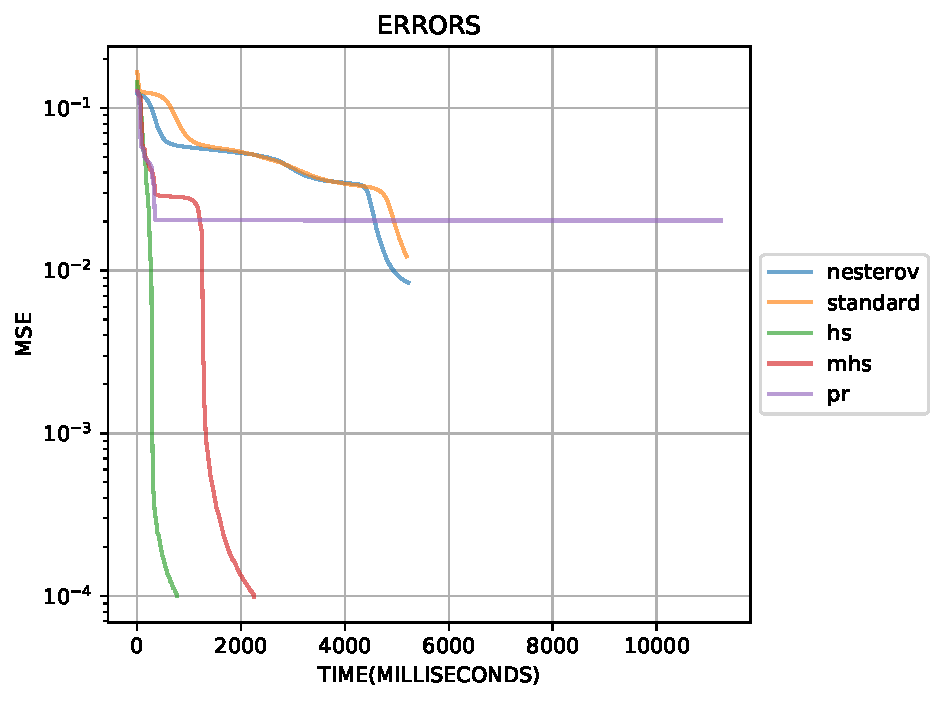
\includegraphics{img/comparisons/1_mse_all_time.pdf}
                    }
                    \caption{}
                    \label{fig:monks_1_MSE_all}
                \end{subfigure}
                \begin{subfigure}{0.40\textwidth}
                    \resizebox{\textwidth}{!}{
                        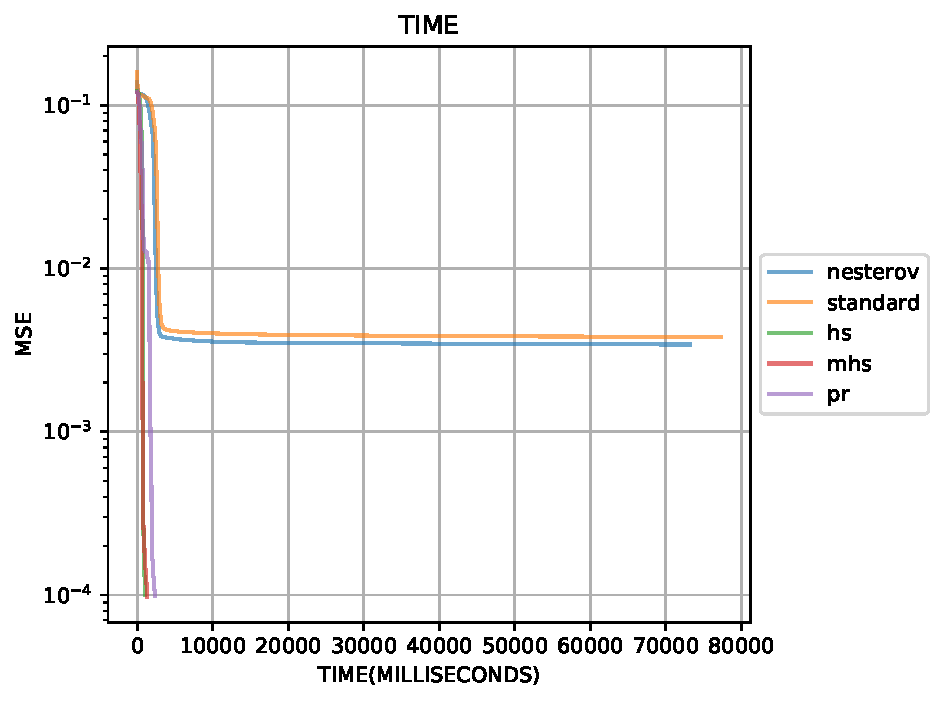
\includegraphics{img/comparisons/2_mse_all_time.pdf}
                    }
                    \caption{}
                    \label{fig:monks_2_MSE_all}
                \end{subfigure}
                \begin{subfigure}{0.40\textwidth}
                    \resizebox{\textwidth}{!}{
                        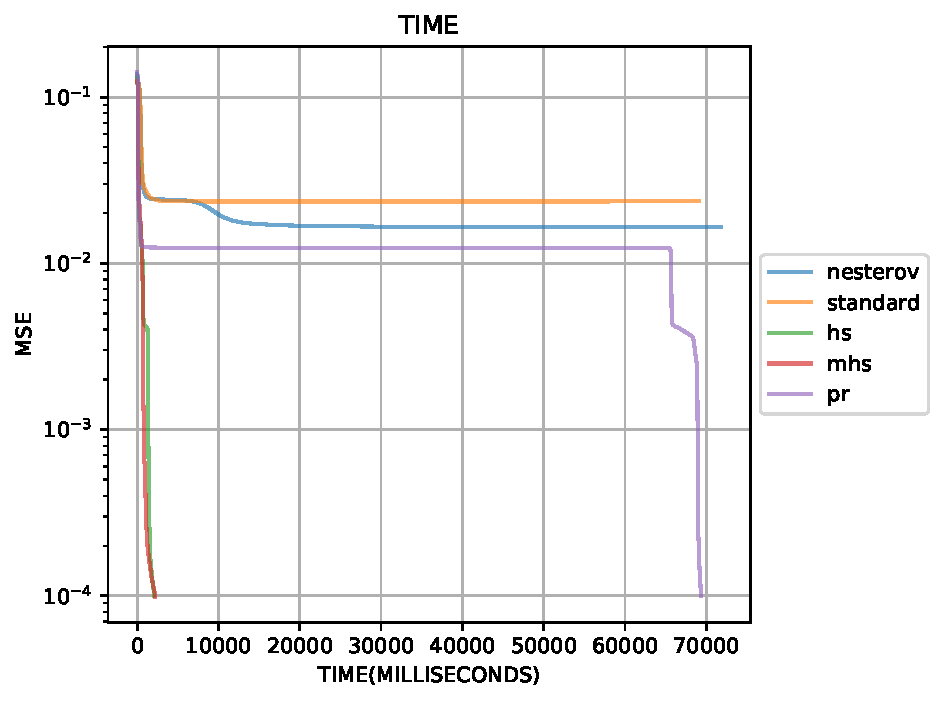
\includegraphics{img/comparisons/3_mse_all_time.pdf}
                    }
                    \caption{}
                    \label{fig:monks_3_MSE_all}
                \end{subfigure}
                \caption{Comparisons between the diffent optimizers without the constrain of setting a maximal
                number of epochs for the iterations. In Figure \ref{fig:monks_1_MSE_all} we can see the
                comparison for MONKS 1, while in Figure \ref{fig:monks_2_MSE_all} we can see the one for
                MONKS 2 and finally in Figure \ref{fig:monks_3_MSE_all} we can see the one for MONKS 3.}
                \label{fig:monks_MSE_all}
            \end{figure}

        % subsection results_ (end)

        \subsection{Results (max epochs 1000)} % (fold)
        \label{sub:results_}

            \begin{table}[H]
                \centering
                \begin{subtable}{\textwidth}
                    \resizebox{\textwidth}{!}{
                        \begin{tabular}{| c | c | c | c | c | c | c | c | c | c | c |}
                            \hline
                            Task & Optimizer & $\beta$ & $\sigma_{1}$ & $\sigma_{2}$ & $\rho$ & $\eta$
                            & $\alpha$ & $\lambda$ & MSE (TR - TS) & Accuracy (TR - TS) (\%) \\
                            \hline
                            MONK 1 & SGD (CM) & - & - & - & - & - & - & - & - & - \\
                            \hline
                            MONK 1 & SGD (NAG) & - & - & - & - & - & - & - & - & - \\
                            \hline
                            MONK 1 & CGD ($PR^{+}$) & - & - & - & - & - & - & - & - & - \\
                            \hline
                            MONK 1 & CGD ($HS^{+}$) & - & - & - & - & - & - & - & - & - \\
                            \hline
                            MONK 1 & CGD ($MHS^{+}$) & - & - & - & - & - & - & - & - & - \\
                            \hline
                            MONK 2 & SGD (CM) & - & - & - & - & - & - & - & - & - \\
                            \hline
                            MONK 2 & SGD (NAG) & - & - & - & - & - & - & - & - & - \\
                            \hline
                            MONK 2 & CGD ($PR^{+}$) & - & - & - & - & - & - & - & - & - \\
                            \hline
                            MONK 2 & CGD ($HS^{+}$) & - & - & - & - & - & - & - & - & - \\
                            \hline
                            MONK 2 & CGD ($MHS^{+}$) & - & - & - & - & - & - & - & - & - \\
                            \hline
                            MONK 3 & SGD (CM) & - & - & - & - & - & - & - & - & - \\
                            \hline
                            MONK 3 & SGD (NAG) & - & - & - & - & - & - & - & - & - \\
                            \hline
                            MONK 3 & CGD ($PR^{+}$) & - & - & - & - & - & - & - & - & - \\
                            \hline
                            MONK 3 & CGD ($HS^{+}$) & - & - & - & - & - & - & - & - & - \\
                            \hline
                            MONK 3 & CGD ($MHS^{+}$) & - & - & - & - & - & - & - & - & - \\
                            \hline
                        \end{tabular}
                    }
                \end{subtable}
                \caption{Comparisons between the iterations having maximal number of epochs egual to 1000.
                Each one of the iterations has been completed with a network having topology
                17 -> 4 -> 8 -> 1.}
                \label{tab:monks_max_epochs}
            \end{table}

        % subsection results_ (end)

        \subsection{Results for Stochastic Gradient Descent} % (fold)
        \label{sub:results_for_stochastic_gradient_descent}

            \begin{table}[H]
                \centering
                \begin{subtable}{\textwidth}
                    \resizebox{\textwidth}{!}{
                        \begin{tabular}{| c | c | c | c | c | c | c | c |}
                            \hline
                            Task & Topology & Momentum & $\eta$ & $\alpha$ & $\lambda$
                            & MSE (TR - TS) & Accuracy (TR - TS) (\%) \\
                            \hline
                            MONK 1 & 17 -> 4 -> 8 -> 1 & standard & 0.65 & 0.75 & 0.0 & 0.010 - 0.016 &
                            100 \% - 99 \% \\
                            \hline
                            MONK 2 & 17 -> 4 -> 8 -> 1 & standard & 0.71 & 0.89 & 0.0 & 0.0072 - 0.010 &
                            100 \% - 100 \% \\
                            \hline
                            MONK 3 & 17 -> 4 -> 8 -> 1 & standard & 0.67 & 0.85 & 0.0027
                            & 0.012 - 0.014 & 98 \% - 98 \% \\
                            \hline
                            MONK 1 & 17 -> 4 -> 8 -> 1 & nesterov & 0.63 & 0.73 & 0.0 & 0.016 - 0.024 &
                            98 \% - 98 \% \\
                            \hline
                            MONK 2 & 17 -> 4 -> 8 -> 1 & nesterov & 0.64 & 0.85 & 0.0 & 0.010 - 0.014 &
                            99 \% - 99 \% \\
                            \hline
                            MONK 3 & 17 -> 4 -> 8 -> 1 & nesterov & 0.61 & 0.76 & 0.0036
                            & 0.014 - 0.016 & 98 \% - 98 \% \\
                            \hline
                        \end{tabular}
                    }
                \end{subtable}
                \caption{Results for the Stochastic Gradient Descent.}
                \label{tab:monks_sgd}
            \end{table}

            In order to compare the results in a similar configuration between the SGD and the CG, we have decided to
            adopt only the \textit{batch} mode for training the ANN.
            Futhermore, for investigate more about the SGD's performances, we have decided to use both the
            \textit{Nesterov momentum} and the \textit{Standard momentum}, as described in
            \cite{Goodfellow-et-al-2016,Sutskever:2013:IIM:3042817.3043064}, both in the validation and testing phases.
            The regularization constant $\lambda$ is used only in the third dataset, since Monk 3 is the only one among
            the three that has noisy samples.

            \begin{table}[H]
                \centering
                \begin{subtable}{\textwidth}
                    \resizebox{\textwidth}{!}{
                        \begin{tabular}{| c | c | c | c | c | c |}
                            \hline
                            Task & Momentum & Convergence on Epoch & Max Accuracy on Epoch & Elapsed Time & Backpropagation time \\
                            \hline
                            MONK 1 & standard & 1000 & 837 & 5.01 & 2.94\\
                            \hline
                            MONK 2 & standard & 1000 & 607 & 5.27 & 2.99\\
                            \hline
                            MONK 3 & standard & 1000 & 427 & 5.18 & 2.97\\
                            \hline
                            MONK 1 & nesterov & 1000 & 641 & 5.24 & 2.94\\
                            \hline
                            MONK 2 & nesterov & 1000 & 450 & 5.37 & 3.02\\
                            \hline
                            MONK 3 & nesterov & 1000 & 317 & 5.26 & 2.99\\
                            \hline
                        \end{tabular}
                    }
                \end{subtable}
                \caption{Additional statistics for the Stochastic Gradient Descent.}
                \label{tab:additional_monks_sgd}
            \end{table}

            As we can see from Tab. \ref{tab:additional_monks_sgd}, the Nesterov's momentum is, in general, faster
            than the standard one in reaching the epoch in which the accuracy score reaches its maximal value, as
            described in \cite{Goodfellow-et-al-2016,Sutskever:2013:IIM:3042817.3043064}. The value of $1000$ for
            the convergence's epochs has to be interpreted as a non convergence for the task, since $1000$ is the
            maximal number of epochs that we have used for the training and the testing phases. The average time of
            execution of the train and backpropagation phases are computed in seconds. Both the momentum choices
            produce similar results.

        % subsection results_for_stochastic_gradient_descent (end)

        \subsection{Results for Conjugate Gradient Methods} % (fold)
        \label{sub:results_for_conjugate_gradient_method}

        \begin{table}[H]
                \centering
                \begin{subtable}{\textwidth}
                    \resizebox{\textwidth}{!}{
                        \begin{tabular}{| c | c | c | c | c | c | c | c | c |}
                            \hline
                            Task & Topology & Activation & $\beta$ & $\sigma_{1}$ & $\sigma_{2}$ & $\rho$
                            & MSE (TR - TS) & Accuracy (TR - TS) (\%) \\
                            \hline
                            MONK 1 & 17 -> 4 -> 8 -> 1 & sigmoid & $MHS^{+}$ & 0.0001 & 0.12 & 0.85
                            & 0.0059 - 0.0125 & 99 \% - 97 \% \\
                            \hline
                            MONK 2 & 17 -> 4 -> 8 -> 1 & sigmoid & $MHS^{+}$ & 0.0001 & 0.33 & 0.42
                            & 0.0039 - 0.0113 & 99 \% - 97 \% \\
                            \hline
                            MONK 3 & 17 -> 4 -> 8 -> 1 & sigmoid & $MHS^{+}$ & 0.0001 & 0.24 & 0.27
                            & 0.0052 - 0.0169 & 99 \% - 96 \% \\
                            \hline
                            MONK 1 & 17 -> 4 -> 8 -> 1 & sigmoid & $HS^{+}$ & 0.0001 & 0.21 & 0.0
                            & 0.0029 - 0.0057 & 99 \% - 99 \% \\
                            \hline
                            MONK 2 & 17 -> 4 -> 8 -> 1 & sigmoid & $HS^{+}$ & 0.0001 & 0.16 & 0.0
                            & 0.0032 - 0.0078 & 99 \% - 98 \% \\
                            \hline
                            MONK 3 & 17 -> 4 -> 8 -> 1 & sigmoid & $HS^{+}$ & 0.0001 & 0.35 & 0.0
                            & 0.0045 - 0.0151 & 99 \% - 96 \% \\
                            \hline
                            MONK 1 & 17 -> 4 -> 8 -> 1 & sigmoid & $PR^{+}$ & 0.0001 &  0.17 & 0.0
                            & $9.89e-05$ - 0.0069 & 100 \% - 98 \% \\
                            \hline
                            MONK 2 & 17 -> 4 -> 8 -> 1 & sigmoid & $PR^{+}$ & 0.0001 & 0.34 & 0.0
                            & $9.35e-05$ - 0.0048 & 100 \% - 99 \% \\
                            \hline
                            MONK 3 & 17 -> 4 -> 8 -> 1 & sigmoid & $PR^{+}$ & 0.0001 & 0.12 & 0.0
                            & 0.0088 - 0.0118 & 98 \% - 97 \% \\
                            \hline
                        \end{tabular}
                    }
                \end{subtable}
                \caption{Results for the Conjugate Gradient Methods.}
                \label{tab:monks_cgd}
        \end{table}

        For what concernes the results for the Conjugate Gradient Methods, for all the configurations tested,
        the direction has been set to the modified one, since it's the one who gave better results in the
        preliminary tests. It's immediate to see high performances achieved by the all the methods. In this case, the $PR^+$ method performes better than the other methods, getting an higher accuracy and converging before the other ones. On the contrary, the $MHS^+$ method needs more epochs than the others to get to the convergence and to the highest accuracy rate.

        Like in the results obtained from SGD, the third
        dataset tested (Monk 3) gets a little worse performances because of the presence of noise in it.
        Anyway, it's interesting to underline that these models are able to reach higher accuracies with the
        ability to "auto-tune" themeselves, that is without the necessity to modify at hand hyperparameters as the
        learning rate or the the momentum term.

        \begin{table}[H]
                \centering
                \begin{subtable}{\textwidth}
                    \resizebox{\textwidth}{!}{
                        \begin{tabular}{| c | c | c | c | c | c | c | c | c | c |}
                            \hline
                            Task & $\beta$ & Convergence Epoch & Max Accuracy Epoch & LS Iterations & Elapsed Time & BP Time & LS Time & Dir Time \\
                            \hline
                            MONK 1 & $MHS^{+}$ & 348 & 216 & 6 & 5.97 & 0.61 & 2.65 & 0.017\\
                            \hline
                            MONK 2 & $MHS^{+}$ & 258 & 176 & 5 & 4.32 & 0.42 & 1.92 & 0.012\\
                            \hline
                            MONK 3 & $MHS^{+}$ & 428 & 136 & 5 & 6.88 & 0.69 & 3.0 & 0.020 \\
                            \hline
                            MONK 1 & $HS^{+}$ & 260 & 135 & 6 & 5.01 & 2.94 & 1.59 & 0.111\\
                            \hline
                            MONK 2 & $HS^{+}$ & 260 & 117 & 5 & 5.27 & 2.99 & 1.72 & 0.113\\
                            \hline
                            MONK 3 & $HS^{+}$ & 432 & 94 & 5 & 5.18 & 2.97 & 2.81 & 0.194\\
                            \hline
                            MONK 1 & $PR^{+}$ & 151 & 95 & 6 & 2.16 & 0.21 & 0.95 & 0.006\\
                            \hline
                            MONK 2 & $PR^{+}$ & 117 & 75 & 5 & 1.73 & 0.17 & 0.77 & 0.004\\
                            \hline
                            MONK 3 & $PR^{+}$ & 189 & 53 & 5 & 2.84 & 0.28 & 1.24 & 0.008\\
                            \hline
                        \end{tabular}
                    }
                \end{subtable}
                \caption{Additional statistics for the Conjugate Gradient Methods.}
                \label{tab:additional_monks_cgd}
            \end{table}

        From Tab.\ref{tab:additional_monks_cgd}, it's interesting to notice that, in all these configurations, the majority of the execution time is spent performing the Line Search: of course, it's an expensive computation because of the frequent evaluation of the Loss function. Futhermore, the average number of iteration per epochs of the LS is included in a range from 5 to 6 times.

        Another nice behaviour with respect to the one showed in SGD, is evident from the learning curves in
        Appendix \ref{cha:monks_learning_curves}: the Conjugate Gradient Methods reach the highest accuracy in
        the very first epochs, while the Stochastic Gradient Descent needs much more epochs of training to converge
        towards an optimum value.

        This is also evident in the plots of the norm of the gradient, where the SGD get a very smooth curve, but far from the minimum (at least at iteration 1000), meaning there could be still room to an improving. The CG, instead, deals with a very good convergence rate, but with an unregular and nonsmooth behaviour in the curve.

        In the case of CG, the methods have been declared to converge when the norm of the gradient gets a value less than $1e-5$.

        % subsection results_for_conjugate_gradient_method (end)
    % section monks (end)

    \section{CUP} % (fold)
        \label{sec:cup}

        A main difference with respect to the models used for Monk, is the choice of the topology of the Network.
        First of all, in this case, being the final task a regression one in which there are two different values to be predicted, the output layer of the ANN is composed by two neurons of output, each one associated to an identity function.

        Then, after some preliminary trials, we have decided to set the number of the hidden layers to $[16,\ 32]$.

        Of course, as for the Monk dataset, we have performed a validation phase on the CUP dataset, in order to
        discover the best parameters for the network. As described in Sec. \ref{sec:monks}, it has been
        implemented a \textit{3-fold cross validation algorithm} with a (random) \textit{grid search}.
        Table \ref{tab:hyper_cup} shows the ranges in which the searching of the hyperparameters has been carried
        out. Once again, the momentum type chosen is Nesterov, while the direction used in the Conjugate Gradient
        Methods is the modified one.

        \begin{table}[H]
          \centering
          \caption{Hyperparameters' ranges for the random grid search algorithm with SGD and CG.}
          \begin{minipage}{.4\textwidth}
              \centering
              \begin{tabular}{| c | c |}
                    \hline
                    Hyperparameters & Ranges\\
                    \hline
                    $\eta$ & $\left [0.004, 0.2\right ]$ \\
                    \hline
                    $\alpha$ & $[0.5, 0.9]$ \\
                    \hline
                    $\lambda$ & $[0.0003, 0.003]$ \\
                    \hline
              \end{tabular}
          \end{minipage}
          \begin{minipage}{.4\textwidth}
              \centering
              \begin{tabular}{| c | c |}
                    \hline
                    Hyperparameters & Ranges\\
                    \hline
                    $\sigma_2$ & $\left [0.1, 0.4 \right ]$\\
                    \hline
                    $\rho$ & $[0.0, 1.0]$ \\
                    \hline
              \end{tabular}
            \end{minipage}
            \label{tab:hyper_cup}
        \end{table}

        In tables \ref{tab:cup_sgd} and \ref{tab:cup_cgd} are annotated the average results obtained from 10 executions of each one of the best models identified thanks to the validation step.

        \begin{table}[H]
                \centering
                \begin{subtable}{\textwidth}
                    \resizebox{\textwidth}{!}{
                        \begin{tabular}{| c | c | c | c | c | c | c | c |}
                            \hline
                            Model & Topology & Batch size & Activation & $\eta$ & $\alpha$ & $\lambda$
                            & MSE (TR - TS) \\
                            \hline
                            SGD & 10 -> 16 -> 32 -> 2 & batch & identity & 0.084 & 0.79 & 0.0009 & 1.00 - 1.35 \\
                            \hline
                        \end{tabular}
                    }
                \end{subtable}
                \caption{Results for the Stochastic Gradient Descent.}
                \label{tab:cup_sgd}
        \end{table}

        \begin{table}[H]
                \centering
                \begin{subtable}{\textwidth}
                    \resizebox{\textwidth}{!}{
                        \begin{tabular}{| c | c | c | c | c | c | c | c |}
                            \hline
                            $\beta$ & Topology & Batch size & Activation & $\sigma_1$ & $\sigma_2$ & $\rho$
                            & MSE (TR - TS) \\
                            \hline
                            $MHS^+$ & 10 -> -> 16 -> 32 -> 2& batch & identity & 0.0001 & 0.27 & 0.29 & 0.97 - 1.50\\
                            \hline
                            $HS^+$  & 10 ->-> 16 -> 32 -> 2& batch & identity & 0.0001 & 0.39 & 0.0
                            & 0.97 - 1.50  \\
                            \hline
                            $PR^+$  & 10 ->-> 16 -> 32 -> 2& batch & identity & 0.0001 & 0.86 & 0.00
                            & 1.15 - 1.41\\
                            \hline
                        \end{tabular}
                    }
                \end{subtable}
                \caption{Results for the Conjugate Gradient Methods.}
                \label{tab:cup_cgd}
        \end{table}

        As for the experiments with the Monk datasets, we attach the learning curves in Appendix \ref{cha:cup_learning_curves}.
% chapter experiments (end)
